\documentclass[sigconf, screen, authorversion, nonacm, authordraft]{acmart}
% \documentclass[sigconf, screen, authorversion, nonacm]{acmart}

\title{ACM Overleaf Template}

% Authors
\author{Evan McKinney}
\email{evm33@pitt.edu}
\orcid{0000-0002-4865-5458}
\affiliation{%
  \institution{University of Pittsburgh}
  \city{Pittsburgh}
  \state{Pennsylvania}
  \country{USA}
}

\author{Alice Johnson}
\email{alice.johnson@example.com}
\orcid{0000-0001-2345-6789}
\affiliation{%
  \institution{Massachusetts Institute of Technology}
  \city{Cambridge}
  \state{Massachusetts}
  \country{USA}
}

\author{Bob Williams}
\email{bob.williams@example.edu}
\orcid{0000-0002-9876-5432}
\affiliation{%
  \institution{University of California, Berkeley}
  \city{Berkeley}
  \state{California}
  \country{USA}
}

\author{Carlos García}
\email{carlos.garcia@example.edu}
\orcid{0000-0003-5678-1234}
\affiliation{%
  \institution{Yale University}
  \city{New Haven}
  \country{USA}
}

\author{Danielle Smith}
\email{danielle.smith@example.ac.uk}
\orcid{0000-0004-4567-7890}
\affiliation{%
  \institution{University of Oxford}
  \city{Oxford}
  \country{United Kingdom}
}

\author{Emily Chen}
\email{emily.chen@example.cn}
\orcid{0000-0005-7890-2345}
\affiliation{%
  \institution{Tsinghua University}
  \city{Beijing}
  \country{China}
}

\renewcommand{\shortauthors}{McKinney et al.}

\begin{abstract}
Lorem ipsum odor amet, consectetuer adipiscing elit. At id euismod rutrum dolor suscipit aptent class. Viverra tortor sodales nunc condimentum egestas tortor sagittis facilisis. Platea dolor ipsum maximus habitant efficitur odio aliquet placerat pulvinar. Curabitur porta massa; fringilla egestas platea sociosqu. Consequat inceptos ridiculus curabitur fusce vel ultricies. Fermentum cras nibh dignissim eros non eget. Sapien sagittis congue et accumsan ex ullamcorper dictum. Maecenas neque turpis placerat finibus fermentum nam. Integer platea magnis scelerisque aenean urna. Sodales bibendum odio justo turpis sem rhoncus dictum. Est dis libero maecenas; iaculis purus tincidunt sagittis. Aptent pulvinar in porttitor nisl eu nibh habitant sollicitudin. Litora dolor accumsan aptent accumsan orci platea ad magnis.
\end{abstract}

\begin{CCSXML}
<ccs2012>
   <concept>
       <concept_id>10010583.10010786.10010813.10011726</concept_id>
       <concept_desc>Hardware~Quantum computation</concept_desc>
       <concept_significance>500</concept_significance>
       </concept>
 </ccs2012>
\end{CCSXML}
\ccsdesc[500]{Hardware~Quantum computation}
\keywords{Quantum computing, quantum architecture}

% % \usepackage{cite}
% % \usepackage[numbers,sort&compress]{natbib}
% % \usepackage{amsmath,amssymb,amsfonts}
% \usepackage{algorithm}
% \usepackage{algpseudocode}
% \usepackage{graphicx}
% % \usepackage{textcomp}
% \usepackage{subcaption}
% % \usepackage{xcolor}
% % \usepackage[hyphens]{url}
% \usepackage{float}
% \usepackage{fancyhdr}
% % \usepackage[bookmarks=true,breaklinks=true,colorlinks,citecolor=blue,linkcolor=blue,urlcolor=blue]{hyperref}
\usepackage{silence}
\WarningFilter{latex}{Empty bibliography}
% \usepackage{xcolor}
% \usepackage{ifthen}
% \usepackage{mathabx}
% \newboolean{showcomments}
% \setboolean{showcomments}{true}
% \ifthenelse{\boolean{showcomments}}
% { \newcommand{\mynote}[3]{
%      \fbox{\bfseries\sffamily\scriptsize#1}
%         {\small$\blacktriangleright$\textsf{\emph{\color{#3}{#2}}}$\blacktriangleleft$}}}
% { \newcommand{\mynote}[3]{}}
% % One command per author:
% \definecolor{asparagus}{rgb}{.25, .65, .20}
% \newcommand{\evm}[1]{\mynote{EVM}{#1}{asparagus}}
% \newcommand{\iy}[1]{\mynote{IY}{#1}{magenta}}
% \newcommand{\mjh}[1]{\mynote{MJH}{#1}{red}}
% \newcommand{\akj}[1]{\mynote{AKJ}{#1}{blue}}
% \newcommand{\cz}[1]{\mynote{CZ}{#1}{orange}}
% \newcommand{\GF}[1]{\mynote{GF}{#1}{purple}}

\begin{document}

\maketitle


\section{Introduction}

\begin{figure}[t]
    \centering
    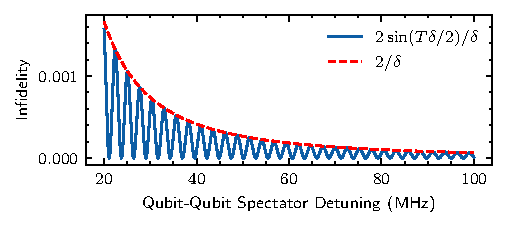
\includegraphics[width=0.95\columnwidth]{figures/fidelity_vs_detuning_up.pdf}
    \caption{Caption.}
    \label{fig:enter-label}
\end{figure}

Lorem ipsum odor amet, consectetuer adipiscing elit. Inceptos lobortis nostra montes volutpat eu ac. Laoreet fusce mi fermentum iaculis adipiscing nam. Aliquet fermentum orci vivamus; erat pulvinar nullam tristique. Donec velit lobortis mus bibendum felis massa. Accumsan blandit non sociosqu ornare nec eleifend. Lacinia fermentum sed mi sed porttitor; eu vitae vulputate. Condimentum sapien lacinia platea nascetur morbi. Facilisis maecenas blandit porttitor nunc integer quam.

Primis sem torquent, eu dignissim eleifend cursus. Non congue et quisque fringilla, rhoncus metus. Inceptos blandit mauris natoque pulvinar eleifend mauris. Euismod a turpis malesuada eleifend lacus massa. Posuere eros ornare habitasse a nostra. Primis nam parturient aenean cubilia, purus sociosqu parturient dapibus vivamus?

Platea nascetur nullam rhoncus laoreet luctus vestibulum id. Potenti aenean quam risus natoque diam velit. Ad montes hac nisl natoque vehicula lorem nullam pellentesque. Luctus conubia nec faucibus feugiat elit himenaeos ex. Conubia lacus torquent nulla, conubia aenean montes turpis. Inceptos interdum ligula adipiscing taciti turpis. Efficitur parturient aptent est sollicitudin mi dignissim vulputate et.

In interdum ullamcorper maximus, orci venenatis lobortis pulvinar condimentum. Morbi neque aenean tortor pellentesque bibendum vulputate commodo. Suscipit quis finibus risus metus etiam pretium. Pretium penatibus augue cursus blandit semper donec neque. Nunc velit enim duis efficitur praesent sapien lectus? Nostra id pulvinar penatibus finibus dignissim sed arcu vestibulum. Sociosqu pulvinar nunc praesent tempor leo aliquet pulvinar odio. Laoreet iaculis nisl molestie lacinia litora turpis ridiculus sodales convallis.

Natoque vitae maximus hendrerit diam conubia cras interdum condimentum vitae. Ut sem elit dolor placerat vestibulum. Duis ad interdum hac quis nisi hendrerit commodo massa. Sollicitudin eget nibh parturient enim mauris elementum sem tincidunt. Vehicula condimentum placerat auctor eu duis penatibus elementum. Sit tristique vel luctus suscipit mi lectus. Neque quis pharetra volutpat diam et magna potenti neque. Turpis facilisi vestibulum ac lorem condimentum. Auctor pellentesque curabitur finibus velit elit lacinia vitae.


\begin{acks}
This work is partially supported by The Charles E. Kaufman Foundation of The Pittsburgh Foundation under New Initiative Award KA2022-129519 and by the Army Research Office under Grants No. W911NF2310253. The views and conclusions contained in this document are those of the authors and should be interpreted as representing official policies, either expressed or implied, of the Army Research Office or the US Government. The US Government is authorized to reproduce and distribute reprints for government purposes notwithstanding any copyright notation herein.
\end{acks}

\bibliographystyle{ACM-Reference-Format}
\nocite{*}
\bibliography{refs}

\end{document}
